\documentclass{article}%
\usepackage[T1]{fontenc}%
\usepackage[utf8]{inputenc}%
\usepackage{lmodern}%
\usepackage{textcomp}%
\usepackage{lastpage}%
\usepackage[head=40pt,margin=0.5in,bottom=0.6in]{geometry}%
\usepackage{graphicx}%
%
\title{\textbf{Protestan en la Concepción Palacios en defensa del contrato colectivo}}%
\author{El Nacional Web}%
\date{16/10/2018}%
%
\begin{document}%
\normalsize%
\maketitle%
\textbf{URL: }%
http://www.el{-}nacional.com/noticias/protestas/protestan{-}concepcion{-}palacios{-}defensa{-}del{-}contrato{-}colectivo\_255937\newline%
%
\textbf{Periodico: }%
EN, %
ID: %
255937, %
Seccion: %
Protestas\newline%
%
\textbf{Palabras Claves: }%
Nicolás Maduro, Salud, Crisis humanitaria, Gobierno\newline%
%
\textbf{Derecho: }%
2.3, %
Otros Derechos: %
, %
Sub Derechos: %
2.3.4\newline%
%
\textbf{EP: }%
SI\newline%
\newline%
%
\textbf{\textit{El personal médico aseguró que el gobierno del presidente Nicolás Maduro no ha atendido sus demandas}}%
\newline%
\newline%
%
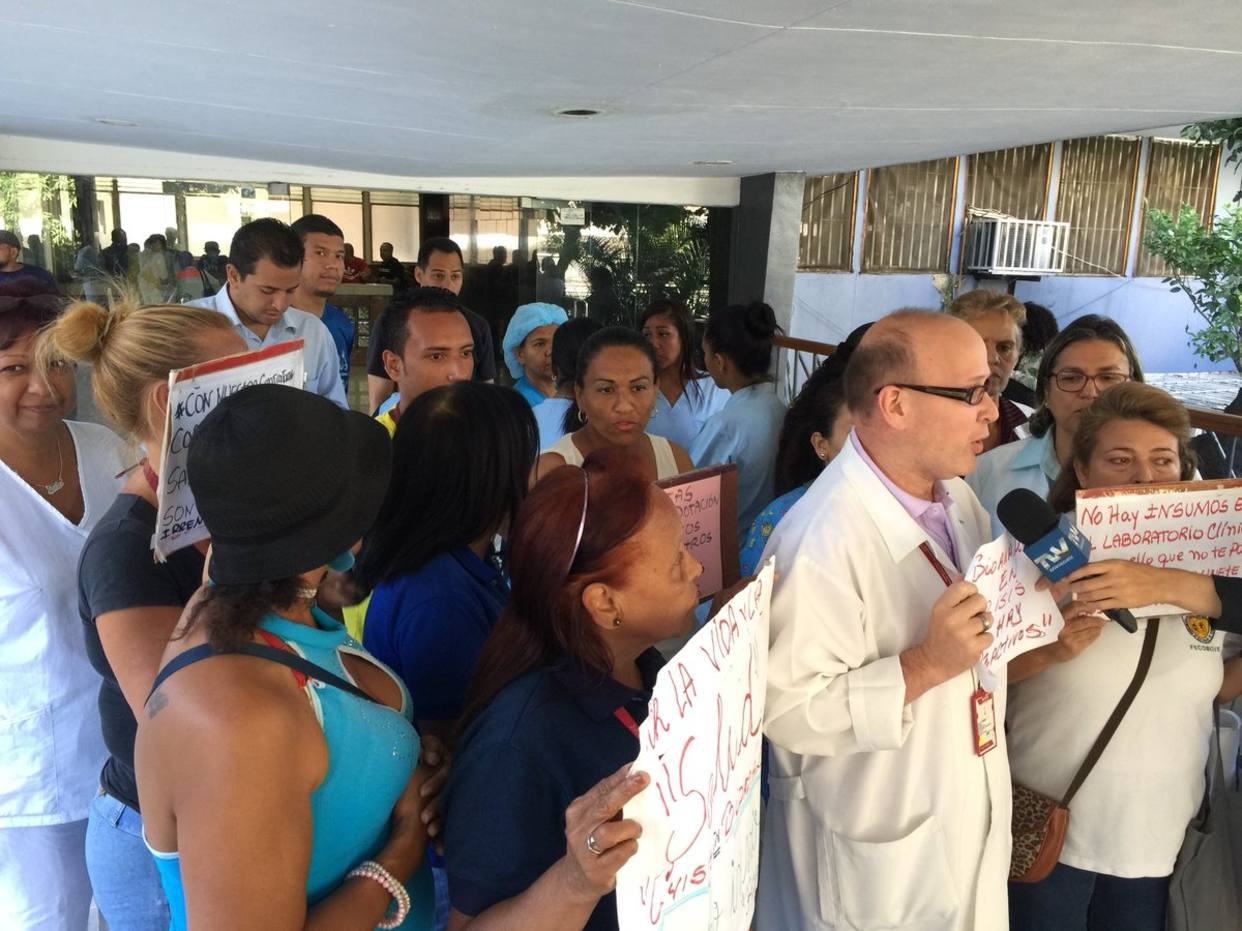
\includegraphics[width=300px]{88.jpg}%
\newline%
%
Trabajadores de la Maternidad Concepción Palacios protestan este martes en defensa del~contrato~colectivo~y mejoras salariales.%
\newline%
%
Denunciaron que la crisis del transporte en el país entorpece el cumplimiento de horario laboral, y las autoridades centro médico sancionan a los empleados.%
\newline%
%
“El paro prácticamente no lo estamos haciendo nosotros. Se nos está obligando a no cumplir con nuestras labores por no tener los insumos necesarios”, manifestó un médico.%
\newline%
%
El personal médico que labora en la Maternidad aseguró que el gobierno del presidente Nicolás Maduro no ha atendido sus demandas.%
\newline%
%
\end{document}